\chapter{Projeto desenvolvido}\label{cap5}

Este capitulo descreve em detalhe o funcionamento do projeto desenvolvido durante o decorrer do estágio.

\section{Funcionamento}

\subsection{Descrição geral}

O \textit{Webshop Service Specification} é uma RESTful API reactiva, que consiste em gerir as especificações de Webshops, ou seja um microserviço reactivo. Este microserviço recebe pedidos HTTP e retorna uma resposta JSON com o resultado, nomeadamente uma Webshop ou uma caraterística da mesma.

Sendo esta API reactiva, ela emprega o uso de \textit{threading} (divisão de tarefas em subprocessos) para poder executar variados pedidos em simultâneo, o mais depressa possível. No entanto esses processos concorrentes e assíncronos requerem um outro nível de cuidado e atenção no que toca à integridade e idempotência dos dados requeridos.

As relações empregues por uma aplicação reactiva são os padrões de \textit{Publisher/Subscriber}, onde um pedido, ou uma transação, é uma mensagem enviada pela fonte desses dados, chamada de um \textit{Publisher} e a sua receção, ou seja onde os dados são consumidos, é encarregado pelo(s) \textit{Subscriber(s)}. Se um desses pedidos for uma mensagem com varias subscrições ao longo do tempo, devemos alterar o \textit{scheduling}, que gere as filas de processos e acessos.

Com isto podemos dizer que os \textit{endpoints} desta API são \textit{Subscribers} e o serviço transacional que comunica diretamente com os dados da base de dados é o nosso \textit{Publisher}. Este tipo de acessos reactivos à base dados requer um outro tipo de mecanismo de processo de transações SQL, o qual deve ser também reactivo de modo a que a base de dados seja vista e funcione com um \textit{Publisher} e seja configurável a sua propagação.

\newpage

Pegando na excelente descrição anterior, o funcionamento deste microserviço pode ser reduzido ao seguinte \textit{flowchart}:

\begin{figure}[!hbt]
  \centering
  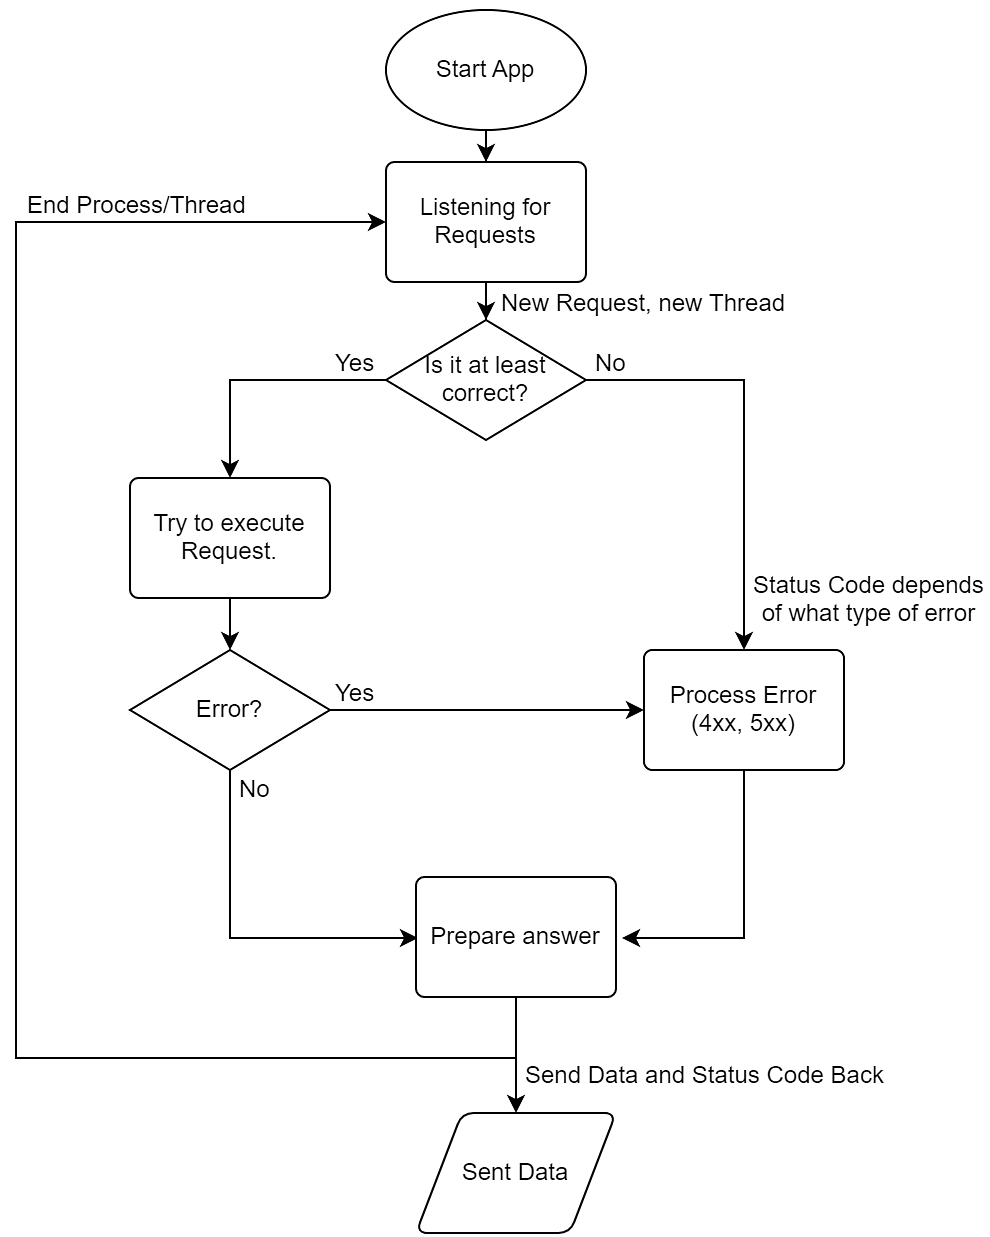
\includegraphics[width=14cm]{figuras/flowchart1.png}
  \caption{\textit{Flowchart} do funcionamento do microserviço, criado no \href{https://gitmind.com/app/flowchart/ccd11723910}{GitMind}}
  \label{fig:flow1}
\end{figure}
\FloatBarrier

Cada um destes processos descritos no \textit{flowchart} (os quadrados), é um objeto ou classe. Os principais vão ser seguidamente descritos com maior detalhe, nas secções seguintes.

\newpage

\section{Organização}

Este projeto (como anteriormente mencionado), é um projeto Gradle que contem dois subprojetos, os quais gerem tarefas diferentes mas co-dependentes:

\begin{itemize}
  \item O pacote dos \hyperref[endp]{\textit{Endpoints}}: um pacote para o core do projeto, este contem a estrutura MC do projeto, com os respectivos modelos, controller e o serviço que comunica com os repositórios do pacote seguinte;
  \item O pacote da \hyperref[infra]{\textit{Infrastructure}}: pacote para os repositórios que tratam das transações com a base de dados e as classes geradas do jOOQ que os repositórios utilizam.
\end{itemize}

Dentro da \textit{root directory} do projeto contemos variadas subdirectorias e ficheiros, dos quais podemos apontar:

\begin{itemize}
  \item \texttt{\textbf{build/ -> }} diretoria onde o Gradle gera os binários, os \textit{jars}, artefactos, etc\ldots da tarefa de compilação;
  \item \texttt{\textbf{endpoints/ -> }} \textit{source directory} do subprojeto \hyperref[endp]{\textit{Endpoints}};
  \item \texttt{\textbf{gradle/ -> }} diretoria onde existem os \textit{wrappers} do Gradle;
  \item \texttt{\textbf{infrastructure/ -> }} \textit{source directory} do subprojeto \hyperref[infra]{\textit{Infrastructure}};
  \item \texttt{\textbf{javadoc/ -> }} diretoria onde se gera o JavaDoc, ou seja um documento/\textit{website} com a documentação (derivada dos \textit{block comments});
  \item \texttt{\textbf{build.gradle -> }} ficheiro de configuração \textbf{principal} do Gradle, onde definimos os pacotes a ir buscar e programamamos as tarefas de (pré e pós) compilação e de testes;
  \item \texttt{\textbf{gradle.properties -> }} ficheiro de configuração \textbf{opcional} do Gradle onde se definem \textit{compiler flags}, argumentos para a JVM e outras configurações mais profundas e especificas;
  \item \texttt{\textbf{lombok.config -> }} ficheiro de configuração \textbf{opcional} do Lombok, onde aqui defino para adicionar a anotação \texttt{@Generated} as suas classes geradas para \textit{fugir} ao JaCoCo;
  \item \texttt{\textbf{micronaut-cli.yml -> }} ficheiro de preferências da criação de um projeto Micronaut via a sua ferramenta CLI;
  \item \texttt{\textbf{postgres-compose.yml -> }} ficheiro de \textbf{docker-compose} para compor e lançar containers com pré configurações, neste caso um container de PostgreSQL;
  \item \texttt{\textbf{settings.gradle -> }} ficheiro de configuração do Gradle onde se definem os subprojetos do projeto Gradle, é executado a cada \textit{build task}.
\end{itemize}

\newpage

\subsection{\textit{\textit{Endpoints} package}}\label{endp}

Este é o subprojeto \textit{Endpoints} onde contêm toda a estrutura base da API, deste o ponto inicial da aplicação, às configurações, modelos, controladores e serviços. Tendo em conta que \texttt{com/optiply/endpoint/} fica como reticências, temos que:

\begin{itemize}
  \item \texttt{\textbf{src/main/}}\begin{itemize}
          \item \texttt{\textbf{java/}}\begin{itemize}
                  \item \texttt{\textbf{\ldots/config/}}\begin{itemize}
                          \item \texttt{\textbf{DataSourceConfig.java}}
                        \end{itemize}
                  \item \texttt{\textbf{\ldots/controllers/}}\begin{itemize}
                          \item \texttt{\textbf{shared/interfaces/IBaseController.java}}
                          \item \texttt{\textbf{shared/BaseController.java}}
                          \item \texttt{\textbf{JSONController.java}}
                        \end{itemize}
                  \item \texttt{\textbf{\ldots/models/}}\begin{itemize}
                          \item \texttt{\textbf{EmailListModel.java}}
                          \item \texttt{\textbf{HandleModel.java}}
                          \item \texttt{\textbf{InterestRateModel.java}}
                          \item \texttt{\textbf{ServiceLevelsModel.java}}
                          \item \texttt{\textbf{SettingsModel.java}}
                          \item \texttt{\textbf{UrlModel.java}}
                          \item \texttt{\textbf{WebshopFullModel.java}}
                          \item \texttt{\textbf{WebshopModel.java}}
                          \item \texttt{\textbf{WebshopSettingsModel.java}}
                        \end{itemize}
                  \item \texttt{\textbf{\ldots/services/}}\begin{itemize}
                          \item \texttt{\textbf{RepositoryService.java}}
                        \end{itemize}
                  \item \texttt{\textbf{\ldots/EndpointApplication.java}}
                \end{itemize}
          \item \texttt{\textbf{resources/}}\begin{itemize}
                  \item \texttt{\textbf{db/migration/}}\begin{itemize}
                          \item \texttt{\textbf{V1\_\_create\_initial\_schema.sql}}
                        \end{itemize}
                  \item \texttt{\textbf{application.yaml}}
                  \item \texttt{\textbf{bootstrap.yaml}}
                  \item \texttt{\textbf{logback.xml}}
                \end{itemize}
        \end{itemize}
\end{itemize}

\newpage

\begin{itemize}
  \item \texttt{\textbf{src/test/}}\begin{itemize}
          \item \texttt{\textbf{java/}}\begin{itemize}
                  \item \texttt{\textbf{integration/}}\begin{itemize}
                          \item \texttt{\textbf{\ldots/controllers/JSONControllerIntegrationTests.java}}
                        \end{itemize}
                  \item \texttt{\textbf{shared/}}\begin{itemize}
                          \item \texttt{\textbf{\ldots/container/TestContainer.java}}
                          \item \texttt{\textbf{\ldots/environment/TestEnvironment.java}}
                        \end{itemize}
                  \item \texttt{\textbf{unit/}}\begin{itemize}
                          \item \texttt{\textbf{\ldots/models/WebshopFullModelsUnitTests.java}}
                          \item \texttt{\textbf{\ldots/services/RepositoryServiceUnitTests.java}}
                        \end{itemize}
                \end{itemize}
          \item \texttt{\textbf{resources/}}\begin{itemize}
                  \item \texttt{\textbf{application-test.yaml}}
                \end{itemize}
        \end{itemize}
\end{itemize}

Sendo que é clara a funcionalidade de cada classe pelo nome e pelo local onde se encontra. Mesmo sendo esse o caso, seguimos para uma explicação breve do que cada classe ou ficheiro faz, excluindo as classes de modelos, pois são obviamente modelos dos objetos transacionais (os corpos em JSON do \textit{request} HTTP) ou de suas partes.

\subsubsection*{\texttt{DataSourceConfig.java}}

Esta classe executa o carregamento e pós-configuração das configurações do ficheiro de configuração \texttt{application.yaml}, criando o contexto DSL (uma interface de comunicação do jOOQ com a base de dados via JDBC), e consequentemente cria a \textit{ConnectionFactory}, que permite usar R2DBC e fazer queries transacionais de forma reactiva.

\subsubsection*{\texttt{JSONController.java}}

Esta classe é um controlador de \textit{requests} HTTP com \textit{payloads} em JSON. Esta, extende a classe de controlador base \texttt{BaseController.java} (abstrata), que por si é uma implementação da interface \texttt{IBaseController.java}, que contem as funções der \textit{parsing} dos parâmetros de procura e sorteamento do \textit{endpoint} de pesquisa de Webshops.

\subsubsection*{\texttt{RepositoryService.java}}

Esta classe é responsável por deter toda a \textit{business logic} necessária e acessível pelos \textit{controllers} e que os isola de contacto direto com os repositórios de dados. É aqui que se executam as tarefas que queremos executadas e recebemos os resultados quando usamos os \textit{endpoints} do \textit{controller}.

\newpage

\subsubsection*{\texttt{EndpointApplication.java}}

Classe principal/base de onde executa a aplicação.

\subsubsection*{\texttt{application.yaml}}

Ficheiro de configurações da aplicação (referido anteriormente \texttt{DataSourceConfig.java}). É aqui onde temos configurações da framework, como o uso do FlyWay, do jOOQ, configurações da fonte de dados (base de dados) e dos meios como lhe comunica (JDBC e R2DBC).

\subsubsection*{\texttt{application-test.yaml} \textsuperscript{\textit{Testes}}}

Semelhante ao anterior, em funcionalidade e não só em nome, são as configurações especificas a ser usadas quando executamos testes. Assim podendo escolher meios de segregar ambientes e containers de teste, ou ajustar recursos de sistema. Neste caso, foi para usar containers de teste novos por cada novo \textit{set} de testes, via TestContainers.

\subsubsection*{\texttt{TestContainer.java} \textsuperscript{\textit{Testes}}}

Classe que configura o lançamento de uma nova instância de um container PostgreSQL (sobre TestContainers) para ser usado como container de testes.

\subsubsection*{\texttt{TestEnvironment.java} \textsuperscript{\textit{Testes}}}

Classe que abstrai o funcionamento da classe anterior quando esta for instanciada qualquer classe de testes que a extenda. Sendo que todas as classes de testes extendem esta classe, ou seja, estão sobre o mesmo ambiente de testes.

\subsubsection*{\texttt{JSONControllerIntegrationTests.java} \textsuperscript{\textit{Testes}}}

Para fazer os testes de integração, testes que testam todo um funcionamento ou percurso não isolado de um processo do projeto, apenas precisamos de fazer testes ao \textit{controller}. Fazendo com que este esteja a receber pedidos HTTP e a escutar as respostas que ele dá, verificando se os resultados obtidos são os esperados.

\subsubsection*{\texttt{WebshopFullModelsUnitTests.java} \textsuperscript{\textit{Testes}}}

Qualquer processo que ocorra nesta aplicação, é um processo de \textit{messaging}, em que o conteúdo das mensagens é dados de um modelo ou o modelo em si, se queremos ter a certeza que estas mensagens ocorrem de forma esperada temos de testar os modelos que elas comunicam. Esta classe faz testes unitários a cada modelo incluso neste projeto.

\subsubsection*{\texttt{RepositoryServiceUnitTests.java} \textsuperscript{\textit{Testes}}}

O serviço neste projeto é o \textit{middleware} que ofusca o \textit{business logic}, como também serve como a comunicação entre os pontos de entrada e o repositório dados que contem o que é pedido, aqui estão definidos os fluxos reactivos das tarefas a fazer. É preciso fazer testes unitários a este serviço, usando o Mockito para imitar comportamentos de classes e objetos que este comunique para isolar o \textit{scope} dos testes.

\subsubsection*{\texttt{V1\_\_create\_initial\_schema.sql}}

Ficheiro \texttt{.sql} com o esquema inicial da base de dados, onde o Gradle executa uma tarefa com o pacote FlyWay para fazer a migração. Esta base de dados contêm duas tabelas, uma com Webshops e as suas caraterísticas e outra para os emails de contacto das Webshops, relação de um-para-muitos.

\subsection{\textit{\textit{Infrastructure} package}}\label{infra}

O subprojeto do \textit{Infrastructure} é onde toda a lógica de comunicação com a base de dados está instalada, desde as classes autogeradas do jOOQ aos repositórios, que são as classes que visam o isolamento e abstração das transações SQL com os que requerem que sejam executadas, nomeadamente o serviço no subprojeto anterior.

\begin{itemize}
  \item \texttt{\textbf{src/main/java/\ldots/data}}\begin{itemize}
          \item \texttt{\textbf{repositories/}}\begin{itemize}
                  \item \texttt{\textbf{interfaces/}}\begin{itemize}
                          \item \texttt{\textbf{IWebshopemailsRepository.java}}
                          \item \texttt{\textbf{IWebshopRepository.java}}
                        \end{itemize}
                  \item \texttt{\textbf{WebshopemailsRepository.java}}
                  \item \texttt{\textbf{WebshopRepository.java}}
                \end{itemize}
          \item \texttt{\textbf{support/sql/}}\begin{itemize}
                  \item \texttt{\textbf{QueryResult.java}}
                \end{itemize}
          \item \texttt{\textbf{package-info.java}}
          \item \texttt{\textbf{resources/}}\begin{itemize}
                  \item \texttt{\textbf{jooq\_schema.sql}}
                \end{itemize}
        \end{itemize}
\end{itemize}

Aqui contem artefactos peculiares, dos quais interfaces para cada Repositório, uma classe de Enums, um ficheiro SQL e um \textit{package-info}. Estes vãos ser seguidamente explicados, tal como no capitulo anterior.

\newpage

\subsubsection*{\texttt{IWebshopRepository.java}}

Interface para implementação do repositório que faz as operações CRUD da tabela de Webshops. Esta interface permite ao Mockito interpretar o comportamento a imitar da classe \texttt{WebshopRepository}.

\subsubsection*{\texttt{IWebshopemailsRepository.java}}

Semelhante à anterior mas para a tabela de emails das Webshops. 

\subsubsection*{\texttt{WebshopRepository.java}}

Classe de operações CRUD reactivas, esta é a classe usada pelo serviço quando necessita de fazer operações na tabela de Webshops.

\subsubsection*{\texttt{WebshopemailsRepository.java}}

Semelhante à anterior mas para operações na tabela de emails das Webshops.

\subsubsection*{\texttt{QueryResult.java}}

Enum de resultados das queries SQL, permitindo fazer operações de equivalência a \textit{result codes} e \textit{status}.

\subsubsection*{\texttt{jooq\_schema.sql}}

Ficheiro com o esquema da base de dados em SQl para que o jOOQ possa criar todas as classes e sistemas referentes à base de dados que é usada. Desde POJOs para usar como objetos transacionais como DAOs e \textit{Specific Result Sets}.

\subsubsection*{\texttt{package-info.java}}

Classe que é interpretada pela framework e que têm apenas como objetivo obrigar a que os parâmetros seja \textit{Nullable by default}. Esta configuração foi herdada pelo estado inicial do projeto.

\newpage

\section{Código}

Nesta seguinte secção vai ser vista em maior detalhe algumas classes e o seu funcionamento especifico, como também explicada algumas decisões po detrás das escolhas feitas sobre o que foi (e como foi) construído.

\subsection{\textit{JSON Controller}}

\subsection{\textit{Webshop Service}}

\subsection{Modelos}

\subsubsection*{Modelos \textit{Webshop\ldots}}

\subsubsection*{Restantes modelos}

\subsection{Repositórios}

\subsubsection*{\texttt{WebshopRepository}}

\subsubsection*{\texttt{WebshopemailsRepository}}

\newpage